\documentclass[12pt,letterpaper]{article}



%%
%% Required packages:
%%
\usepackage{etex}
\usepackage{amsmath}
\usepackage{amssymb}
\usepackage{amstext}
\usepackage{amsthm}
\usepackage{fancyhdr,fancybox}
\usepackage{mathrsfs} % need for \mathscr command
\usepackage{multicol}
\usepackage[normalem]{ulem}
%\usepackage{pictex,pictexplus}
% \usepackage{pictexwd}
\usepackage{rotating}
\usepackage{url}
\usepackage{xfrac}
\usepackage{booktabs}
\usepackage{color,soul}
\usepackage{comment}

\usepackage{hyperref}
\hypersetup{
    colorlinks=true,     % false: boxed links; true: colored links
    linkcolor=blue,      % color of internal links
    citecolor=blue,      % color of links to bibliography
    filecolor=blue,      % color of file links
    urlcolor=blue        % color of external links
}


\usepackage{tikz}
\usetikzlibrary{backgrounds,calc}

%%
%% Common formatting commands
%%
\setlength{\parindent}{0in}
\setlength{\textwidth}{7in}
\setlength{\evensidemargin}{-0.25in}
\setlength{\oddsidemargin}{-0.25in}
\setlength{\parskip}{.5\baselineskip}
\setlength{\topmargin}{-0.5in}
\setlength{\textheight}{9in}

%               Problem and Part
\newcounter{problemnumber}
\newcounter{partnumber}
\newcounter{subpartnumber}
\newcommand{\Problem}{%
  \refstepcounter{problemnumber}%
  \setcounter{partnumber}{0}%
  \setcounter{subpartnumber}{0}%
  \item[\makebox{\hfil\textbf{\theproblemnumber.}\hfil}]%
  }
\newcommand{\InProblem}[2][1.6]{%
  \refstepcounter{problemnumber}%
  \setcounter{partnumber}{0}%
  \setcounter{subpartnumber}{0}%
  \textbf{\theproblemnumber.}\ \ \parbox[t]{#1in}{#2}%
}
\newcommand{\InSmallProblem}[1]{\InProblem[1.05]{#1}}
\newcommand{\NoProblem}[1]{%
  \mbox{\hfil\textbf{#1}\hfil}%
  }
\newcommand{\UnProblem}{%
  \refstepcounter{problemnumber}%
  \setcounter{partnumber}{0}%
  \setcounter{subpartnumber}{0}%
  \mbox{\hfil\textbf{\theproblemnumber.}\hfil}%
  }
\newcommand{\InFlexProblem}[1]{%
  \refstepcounter{problemnumber}%
  \setcounter{partnumber}{0}%
  \setcounter{subpartnumber}{0}%
  \textbf{\theproblemnumber.}\ \ #1%
}
%%  Part:
\newcommand{\Part}{%
  \renewcommand{\thepartnumber}{(\alph{partnumber})}%
  \refstepcounter{partnumber}
  \setcounter{subpartnumber}{0}%
  \item[(\alph{partnumber})]%
}
\newcommand{\InPart}[2][1.75]{%
  \renewcommand{\thepartnumber}{(\alph{partnumber})}%
  \refstepcounter{partnumber}%
  \setcounter{subpartnumber}{0}%
  (\alph{partnumber})\ \ \parbox[t]{#1in}{#2}%
}
\newcommand{\UnPart}{%
  \refstepcounter{partnumber}%
  \renewcommand{\thepartnumber}{(\alph{partnumber})}%
  \setcounter{subpartnumber}{0}%
  (\alph{partnumber})%
}
\newcommand{\InLargePart}[1]{\InPart[3.05]{#1}}
\newcommand{\InFullPart}[1]{\InPart[6.2]{#1}}
\newcommand{\InSmallPart}[1]{\InPart[1.05]{#1}}
%% SubPart:
\newcommand{\SubPart}{%
  \refstepcounter{subpartnumber}%
  \item[(\roman{subpartnumber})]%
  }
\newcommand{\InSubPart}[2][2.25]{%
  \stepcounter{subpartnumber}%
  (\roman{subpartnumber})\ \ \parbox[t]{#1in}{#2}%
}
\newcommand{\InSmallSubPart}[1]{\InSubPart[1.5]{#1}}
\newcommand{\InTinySubPart}[1]{%
  \stepcounter{subpartnumber}%
  (\roman{subpartnumber})\ \ \makebox{#1}%
}
\newcommand{\InMySubPart}[2][2.25]{%
  \stepcounter{subpartnumber}%
  \parbox[t]{#1in}{\makebox[0.3in][l]{(\roman{subpartnumber})}\ \ {#2}}%
}
\newcommand{\TrueFalse}{\textbf{T}\ \ \textbf{F}\ \ }
\newcommand{\TFPart}[1]{% 
  \stepcounter{partnumber}%
  \setcounter{subpartnumber}{0}%
  \item[(\alph{partnumber})] \TrueFalse\parbox[t]{5.5in}{#1}}

\newcommand{\Points}[1]{(#1 points) \ }
\newcommand{\Point}[1]{(#1 point) \ }


%% For Answers:
\newcounter{answernumber}
\newcommand{\Answer}{%
  \refstepcounter{answernumber}%
  \setcounter{partnumber}{0}%
  \setcounter{subpartnumber}{0}%
  \item[\makebox{\hfil\textbf{\theanswernumber.}\hfil}]%
  }


% Setting up the headers for the first page
%\chead{} % will default to what is typed in the file.
\fancyhead[L]{\textsc{Math 22a}}
\fancyhead[R]{\textsc{Fall 2024}}
\fancyfoot[R]{
	\vspace*{\fill}\footnotesize\textcopyright{} \emph{Harvard Math 22a}	
}
\renewcommand{\headrulewidth}{0pt}

%\fancyhead[C]{}
%	\chead{}	
%	\lhead{}
%	\rhead{}
%	\cfoot{}


% Putting copyright on the footer of each page
%\fancypagestyle{secondpage}{
%	\fancyhead[C]{TESTing again} % change this to be blank
%		%\chead{}	
%	\fancyhead[L]{bears} % change this to be blank
%	\fancyhead[R]{dogs} % change this to be blank
%	\fancyfoot[R]{ %keeps the footer the same
%		\vspace*{\fill}\footnotesize\textcopyright{} \emph{Harvard Math 22a}	
%	}
%}
%\renewcommand{\headrulewidth}{0pt}
%\pagestyle{fancy}
\pagestyle{empty}


%\lhead{}
%\rhead{}
%\rfoot{\vspace*{\fill}\footnotesize\textcopyright{} \emph{Harvard Math 22a}}
%\renewcommand{\headrulewidth}{0pt}
%\pagestyle{fancy}




%%
%% Common shortcut commands:
%%
\newcommand{\ds}{\displaystyle}
\newcommand{\sgn}{\operatorname{sgn}}
\renewcommand{\Pr}{\operatorname{P}}
\newcommand{\CPr}[3][{}]{\Pr_{\text{#1}}\left(#2\,|\,#3\right)}

\newcommand{\C}{\mathbb{C}}
\newcommand{\R}{\mathbb{R}}
\newcommand{\Z}{\mathbb{Z}}
\newcommand{\N}{\mathbb{N}}
\newcommand{\Q}{\mathbb{Q}}
\newcommand{\D}{\mathbb{D}}

\newcommand{\rref}{\operatorname{rref}}
\newcommand{\im}{\operatorname{im}}
\newcommand{\rank}{\operatorname{rank}}
\newcommand{\diag}{\operatorname{diag}}
\newcommand{\Span}{\operatorname{span}}
%\renewcommand{\vec}[1]{\mathbf{#1}}
\newcommand{\charpoly}{\mathscr{P}}
\newcommand{\nicefrac}[2]{\sfrac{#1}{#2}} % using xfrac package
\newcommand{\topology}{\mathcal{T}}
\newcommand{\Inn}{\operatorname{Inn}}

\newcommand{\blankbox}[2]{\fbox{\rule{#1}{0in}\rule{0in}{#2}}}

\newenvironment{myindentpar}[1]%
 {\begin{list}{}%
         {\setlength{\leftmargin}{#1}
          \setlength{\rightmargin}{\leftmargin}}%
         \item[]%
 }
 {\end{list}}
\newtheorem{theorem}{Theorem}
\newtheorem*{NStheorem}{Theorem}
\newtheorem{cor}[theorem]{Corollary}
\newtheorem*{claim}{Claim}
\newtheorem{defn}{Definition}

\newenvironment{amatrix}[1]{%
  \left(\begin{array}{@{}*{#1}{c}|c@{}}
}{%
  \end{array}\right)
}

%--------grstep
% For denoting a Gauss' reduction step.
% Use as: \grstep{\rho_1+\rho_3} or \grstep[2\rho_5 \\ 3\rho_6]{\rho_1+\rho_3}
\newcommand{\grstep}[2][\relax]{%
   \ensuremath{\mathrel{
       {\mathop{\longrightarrow}\limits^{#2\mathstrut}_{
                                     \begin{subarray}{l} #1 \end{subarray}}}}}}
\newcommand{\swap}{\leftrightarrow}


\usetikzlibrary{arrows}
\usepackage{wrapfig}

\makeatletter
\renewcommand*\env@matrix[1][*\c@MaxMatrixCols c]{%
	\hskip -\arraycolsep
	\let\@ifnextchar\new@ifnextchar
	\array{#1}}
\makeatother

\def\env@matrix{\hskip -\arraycolsep
	\let\@ifnextchar\new@ifnextchar
	\array{*\c@MaxMatrixCols c}}

\chead{\Large\textbf{Geometry of Determinants, $\vec\S$3.2, 3.3}}% 

\begin{document}
\thispagestyle{fancy}

Recall from last class:

\begin{itemize}
\item For a matrix $A$, define  $A_{ij}$ to be the matrix obtained from $A$ by deleting row $i$ and column $j$.
\item For $n\geq 2$, the determinant of an $n\times n$ matrix $A=[a_{ij}]$ is
\begin{equation*}
\operatorname{det}(A)= a_{11} \operatorname{det}(A_{11}) - a_{12} \operatorname{det}(A_{12})+\dots + (-1)^{n+1} a_{1n} \operatorname{det}(A_{1n})=\sum_{j=1}^{n}(-1)^{1+j}a_{1j} \operatorname{det}(A_{1j}).
\end{equation*} We call this the cofactor expansion across the first row.
\item {\bf Mohan's Theorem:} Cofactor expansion across any row or column is the same, and hence each cofactor expansion gives the determinant.
\item Let $A=[a_{ij}]$ be an $n\times n$ matrix, then $A$ is {\bf upper triangular} if $a_{ij}=0$ when $i>j$.
{\bf Theorem 3.2:} Let $A$ be an $n\times n$ upper triangular matrix, then $$\operatorname{det}(A)= a_{11}a_{22}\dots a_{nn} = \prod_{j=1}^n a_{jj}.$$
\item {\bf Theorem 3.3:} If $A$ is an $n\times n$ matrix and $E$ is an elementary matrix, then $$\operatorname{det}(EA)=\operatorname{det}(E) \operatorname{det}(A),$$ and 
$$\operatorname{det}(E)=\begin{cases}
1 & \text{if $E$ represents adding a multiple of a row to another row,}\\
-1 & \text{if $E$ represents interchanging two rows,}\\
r & \text{if $E$ represents scaling a row by a factor of $r$.}
\end{cases}$$
\end{itemize}

\newpage

{\bf Theorem 3.6:} If $A$ and $B$ are $n$ by $n$ matrices, then $$\operatorname{det}(AB)=\operatorname{det}(A)\operatorname{det}(B).$$

\begin{enumerate}



\Problem Prove the theorem.

\vfill
\vfill

\Problem {\bf Corollary:} $A$ is invertible if and only if $\operatorname{det}(A)\neq0$. Prove the corollary.

\vfill

\newpage

\Problem {\bf True or False:} 

\Part If $A$ is an $n\times n$ invertible matrix, then $\operatorname{det}(A^{-1})=\frac{1}{\operatorname{det}(A)}$.

\vfill

\Part If $A$ is an $n\times n$ matrix, then $\operatorname{det}(A)=\operatorname{det}(A^{T})$.

\vfill

\Part If $A \sim B$, then $\operatorname{det}(A)=\operatorname{det}(B)$.

\vfill

\Problem We can think of $\operatorname{det}$ as a function from the set of $n\times n$ matrices to the real numbers. Is this function linear?

\vfill

\newpage


\Problem Let $T:\mathbb{R}^2 \to \mathbb{R}^2$ be given by $T(\vec{x})=A\vec{x}$ where $A=\begin{bmatrix} 2 & 0\\ 0 & 3\\ \end{bmatrix}$. Let $S_1$ be the unit square given by $S_1=\{(x,y) : 0\leq x, y \leq 1\}$. 

\Part Find $T(S_1)$.

\vfill

\Part How does the area of $S_1$ related to the area of $T(S_1)$?

\vfill

\Part Suppose $S_2=\{(x,y) : 0\leq x, y \leq 2\}$. How does the area of $S_2$ related to the area of $T(S_2)$?

\vfill

\newpage

\Problem Let $T:\mathbb{R}^2 \to \mathbb{R}^2$ be given by $T(\vec{x})=A\vec{x}$ where $A=\begin{bmatrix} a & b\\ c & d\\ \end{bmatrix}$. Let $S$ be the unit square given by $S=\{(x,y) : 0\leq x, y \leq 1\}$. 

\Part Find $T(S)$.

\vfill

\Part How does the area of $S$ related to the area of $T(S)$?

\vfill

\newpage

{\bf Theorem:} If $A$ is a $2 \times 2$ matrix, then the area of the parallelogram determined by the columns of $A$ is $|\det{A}|$. If $A$ is a $3 \times 3$ matrix, then the volume of the parallelepiped is $|\det{A}|$.

\Problem Find the area of the parallelogram with vertices $(-1,0)$, $(0,5)$, $(1,-4)$, and $(2,1)$.

\vfill

{\bf Theorem:} Let $T: \mathbb{R}^2 \to \mathbb{R}^2$ be linear with associated matrix $A$. If $S$ is a parallelogram in $\mathbb{R}^2$, then $\text{Area}(T(S))=|\det{A}|\text{Area}(S)$. 


We will generalize this theorem in Math 22b using calculus to more general functions!


%\newpage
%
%\begin{center}
%{\bf Quiz Review Questions}
%\end{center}
%
%\Problem {True or False Questions}
%
%\begin{enumerate}
%\item  If $A$ and $B$ are $n$ by $n$ matrices with $\det(A)=2$ and $\det(B)=3$, then $\det(A+B)=5$.
%\item $k \text{det}(A) = \text{det}(kA)$
%%\item $AB$ is invertible if and only if $A$ and $B$ are invertible.
%\item If $A$ is row-equivalent to $B$, then \text{det}(A)=\text{det}(B).
%\item If $A$ is invertible and $AB=0$, then $B=0$.
%%\item If $T^2(x)=x$, then $T(x)=x$.
%%\item $S$ and $T$ linear transformations.  If $S \circ T$ is one-to-one, then T is one-to-one.  Must $S$ be one-to-one?
%%\item $S$ and $T$ linear transformations.  If $S \circ T$ is onto, then S onto.  Must $T$ be onto?
%\item If $A^2=I_2$, then $A=I$ or $A=-I$.
%\item If $A^2=0$, then $A=0$
%%\item there exists $u,w,u \in \mathbb{R}^3$ linearly dependent, so that none of the 3 is a multiple of another.
%\item $\text{det}(A) = \text{det}(B)$ implies $A-B$ is not invertible.
%%\item Let $M$ be an $n$ by $n$ matrix with $n$ odd.  If $M^{T}=-M$, then $M$ is not invertible.
%%\item If there exists a matrix $C$ so that $A= C^{-1} B C$, then \text{det}(A)=\text{det}(B).
%%\item Let $T : \mathbb{R}^3 \to \mathbb{R}^3$ be rotation around $z$-axis, and $A$ be the standard matrix for $T$, then $\det{A}=1$.
%%\item Let $T : \mathbb{R}^3 \to \mathbb{R}^3$ be projection onto the $yz$-plane, and $A$ be the standard matrix for $T$, then $\det{A}=0$.
%%\item If $A$ is invertible and $A^{T}=-A$, then A is an $n$ by $n$ matrix where $n$ is even.
%\item Let $T(x) =Ax$ and $S(x)=Bx$ and $A \sim B$, then $\text{im}(T) = \text{im}(S)$.
%\item Let $A$ and $B$ have RREF form, then the span of the columns of $A$ equals the span of the columns of $B$.
%%\item If $Ax=b$ has a unique solution, then $A$ is a square matrix.
%%\item If $A^2+4A+3I=0$, and $A$ is 3 by 3, then $A$ is invertible.
%%\item If $A$ is $n$ by $n$ so that $A^2-A=0$, then $A=I$ or $A=0$.
%%\item There is a 2 by 2 matrix $A$ with real entries so that $A^2 = -I$.
%%\item There exists invertible 2 by 2 matrices $A$ and $B$ so that $\det(A+B)=\det(A)+\det(B)$.
%%\item  For any 2 by 2 matrix A, there exists $\lambda \in \mathbb{R}$ so that $A+ \lambda I$ is singular.
%\item  There is a linear transformation $T : \mathbb{R}^2 \to \mathbb{R}^2$ so that $\{ x : T(x)=0 \} = \{ T(x) : x \in \mathbb{R}^2 \}.$
%\item   If $u, v, w$ are pairwise linearly independent, then $u, v, w$ are linearly independent. 
%\end{enumerate}
%
%\Problem 
%\begin{enumerate}	
%\item		Let $T\colon \R^3 \rightarrow \R^3$ be the transformation that scales all vectors by a factor of 3.
%Let $A$ be the standard matrix for $T$.  What is $\det(A)$?
%%\begin{solution}
%%	We have that $T(\vec e_{1})=(3,0,0)$, $T(\vec e_{2})=(0,3,0)$ and $T(\vec e_{3})=(0,0,3)$.
%%	So the standard matrix for $T$ is $A=\begin{bmatrix}3&0&0\\0&3&0\\0&0&3\end{bmatrix}$.
%%	Since $A$ is triangular, the determinant of $A$ is the product of the diagonal entries: $\det(A)=27$.
%%\end{solution}
%%\blank
%%\part[3]
%\item Let $T\colon \R^3 \rightarrow \R^3$ be the transformation that reflects across the plane $x=z$.
%Let $A$ be the standard matrix for $T$.  What is $\det(A)$?
%%\begin{solution}
%%	We have that $T(\vec e_{1})=\vec e_3, T(\vec e_{2})=\vec e_{2}$ and $T(\vec e_{3})=\vec e_{1}$.
%%	So the standard matrix for $T$ is
%%	$A=\begin{bmatrix}0&0&1\\0&1&0\\1&0&0\end{bmatrix}.$ Since $A$ is obtained from the identity
%%	matrix by exchanging the first and third columns, $\det(A)=-1$.
%%\end{solution}
%%\blank
%%\part[3]
%\item Let $T\colon \R^3 \rightarrow \R^3$ be the transformation that projects to the plane $x=z$.
%Let $A$ be the standard matrix for $T$. What is $\det(A)$?
%%\begin{solution}
%%	Since $T$ is not onto $\R^{3}$, $T$ is not invertible. So the standard matrix $A$ for $T$ is not
%%	invertible. Thus, $\det(A)=0$.
%%\end{solution}
%%\blank
%\end{enumerate}

%\Problem 
%
%\begin{enumerate}
%	\item Suppose $A\vec{x} = - \vec{x}$ has only the trivial solution.  Then prove that $$\det (A^2 + 2A + I_n) >0;$$ \textit{i.e.} the determinant is \emph{strictly} positive.
%
%
%
%
%\item  In the previous part, is the assumption that $A\vec{x} = - \vec{x}$ has only the trivial solution necessary?  Either prove the statement without the assumption or give an explicit counterexample to show that it is not possible to drop the assumption.
%
%\end{enumerate}
%
%\Problem Let \begin{equation*}
%A=\begin{bmatrix}
%1 & 0 & 1\\
%3 & 3 & 4\\
%2 & 2 & 3\\
%\end{bmatrix}.
%\end{equation*}  Find $A^{-1}$.
%
%\Problem 
%\begin{enumerate}
%	\item Prove that if $T$ is one-to-one and $\vec{u_1}, \cdots, \vec{u_p}\in \mathbb{R}^n$ are linearly independent, then $T(\vec{u_1}), \cdots, T(\vec{u_p})$ are linearly independent in $\mathbb{R}^m$.
%	\item In part (a), is the hypothesis that $T$ is one-to-one necessary?  Why or why not?
%\end{enumerate}
%
%\Problem Compute the determinant of the following matrices:
%\begin{enumerate}
%	\item
%	\begin{equation*}
%	A_1=\begin{bmatrix}
%	1 & 1\\
%	a_1 & 1\\
%	\end{bmatrix}.
%	\end{equation*}
%	\item 
%	\begin{equation*}
%	A_2=\begin{bmatrix}
%	1 & 1 & 1\\
%	a_1 & 1 & 1\\
%	a_2 & a_1 & 1\\
%	\end{bmatrix}.
%	\end{equation*}
%	\item Find the determinant of the following matrix.  Use induction to prove your formula is correct.
%	\begin{equation*}
%	A_n=\begin{bmatrix}
%	1 & 1 & \cdots & 1 & 1\\
%	a_1 & 1 & \cdots & 1& 1\\
%	\vdots &  & &&\vdots\\
%	a_{n-1} & a_{n-2} &  \ddots &  1    & 1\\
%	a_{n}     & a_{n-1} & \cdots & a_1 & 1\\
%	\end{bmatrix}.
%	\end{equation*}
%\end{enumerate}
%\Problem 
%\begin{enumerate}
%\item Prove $|\mathbb{N}|=|\{0\} \cup \mathbb{N}|$.
%\item Prove $|\mathbb{N}|=|\{-2,-1\} \cup \mathbb{N}|$.
%\item Prove $|[a,b]|=|[c,d]|$.
%\end{enumerate}

\end{enumerate}

\begin{comment}
\newpage
\chead{\Large\textbf{Determinant Geometry -- Answers / Solutions}}%
\lhead{}
\rhead{}
\thispagestyle{fancy}

\begin{enumerate}
  \Answer 
  
  \begin{proof}
  	
  We prove the result by cases.
  
  {\bf Case 1:} $A$ is invertible.
  
  Since $A$ is invertible, the invertible matrix theorem tells us that there exists elementary row operations $E_1, \dots, E_p$ such that $I_n=E_p \dots E_1 A$. Since elementary matrices are invertible and the inverse of an elementary matrix is another elementary matrix, we get $A=E_1^{-1}\dots E_p^{-1}$. Thus we get $AB=E_1^{-1}\dots E_p^{-1}B$. Now we apply the previous theorem multiple times to get the following
  \begin{align*}
  		\det{AB} &=\det{E_1^{-1}\dots E_p^{-1} B}\\
	&= \det{E_{1}^{-1}}\det{E_2^{-1}}\dots\det{E_{p}^{-1}}\det{B}\\
	&= \det{E_1^{-1}\dots E_p^{-1}}\det{B}\\
	&= \det{A}\det{B}.
\end{align*}
  
  {\bf Case 2:} $A$ is not invertible.
  
There must be a sequence of elementary matrices $E_1,\dots, E_p$ such that $A=E_1\dots E_p U$ where $U$ is the reduced row echelon form of $A$. Since $A$ is not invertible, the invertible matrix theorem gives that $U\neq I_n$. Moreover, $U$ must be upper triangular and have a zero along the diagonal. Thus $\det{A}=\det{E_1\dots E_p U}=\det{E_1}\dots \det{E_p}\det{U}=0$ since $\det{U}=0$.

Since $A$ is not invertible, we know $AB$ is not invertible. Thus we can apply the same reasoning to $AB$ to conclude $\det{AB}=0$. Hence $\det{AB}=0=\det{A}\det{B}$.
  \end{proof}
  
  \Answer 
  
  \begin{proof} We prove the two implications.
  	
  $\implies$ Suppose $A$ is invertible, then $AA^{-1}=I_n$. By the previous theorem, $1=\det{A}\det{A^{-1}}$, and hence $\det{A}\neq 0$.
  
  $\impliedby$ Suppose $\det{A}\neq 0$. We know there are elementary matrices $E_1,\dots E_p$ such that $A=E_1\dots E_p U$ where $U$ is the reduced row echelon form of $U$. We know $\det{E_k}\neq 0$ for all $1\leq k \leq p$. Thus $\det{U}\neq 0$. Since $U$ is an upper triangular matrix, we know the determinant of $U$ is the product of the diagonal elements. Thus $U$ cannot have a zero along the diagonal. Thus $U$ has all ones along the diagonal. Since $U$ is a square matrix, we get $U=I_n$. By the invertible matrix theorem, $A$ must be invertible.
  	
  \end{proof}
  
  \Answer 
  
  \begin{enumerate}
  \item {\bf True.} Since $A$ is invertible, we know $AA^{-1}=I_n$. Thus $1=\det{I_n}=\det{AA^{-1}}=\det{A}\det{A^{-1}}$, and hence $\det{A^{-1}}=\frac{1}{\det{A}}$.
  
  \item {\bf True.} Let $a_{ij}$ be the entry in row $i$ and column $j$ of $A$ and let $b_{ij}$ be the entry in row $i$ and column $j$ of $A^{T}$.
  
  Expand the determinant of $A$ along the first column and use $a_{ij}=b_{ji}$; namely, 
 \begin{align*}
 	\det{A}&=a_{11} \det A_{11} -a_{21}\det A_{21}+\dots+(-1)^{n+1} a_{(n+1)1}\det A_{(n+1)1}\\
 	&= b_{11} \det (A^{T})_{11}- b_{12} \det (A^{T})_{12}+\dots +(-1)^{n+1}b_{1n}\det{(A^{T})_{1n}}=\det{A^T}.
  \end{align*}
  
  \item {\bf False.} Let $A=\begin{bmatrix} 1 & 0\\ 0 & 1\\ \end{bmatrix}$ and $B=\begin{bmatrix} 0 & 1\\ 1 & 0\\ \end{bmatrix}$, then $A\sim B$ and $\det{A}=1$ and $\det{B}=-1$.
  \end{enumerate}
  
  \Answer Let $M_{n\times n}$ be the set of $n\times n$ matrices, then $\det : M_{n\times n} \to \mathbb{R}$ is a function. This function fails to be linear since $\det{I_2}=1$ but $\det{2I_2}=4$.
  
  It is worth noting that if we instead defined the function $f_j: \mathbb{R}^n \to \mathbb{R}$ by $\det{[\vec{a}_1 \dots, a_{j-1} \; \vec{x} \; \vec{a}_{j+1} \dots \vec{a}_n]}$, then $f_j$ is linear. Thus the determinant is linear in each column; we call this property {\bf multi-linear}.
  

  \Answer 
  
  \begin{enumerate}
  \item In the figure below, we see how $S_1$ transforms under the transformation $T$.
  
\begin{center}
	\begin{tikzpicture}[
scale=1,
	axis/.style={very thick, ->, >=stealth'},
	important line/.style={thick},
	dashed line/.style={dashed, thin},
	pile/.style={thick, ->, >=stealth', shorten <=2pt, shorten
		>=2pt},
	every node/.style={color=black},
 vertex/.style={circle, minimum size=4pt, inner sep=0pt, fill=orange}
]

\begin{scope}[local bounding box=graph1]
	\draw[axis] (-0.1,0)  -- (3.5,0) node(xline)[right]
	{};
	\draw[axis] (0,-0.1) -- (0,3.5) node(yline)[above] {};
	
	\fill[blue] (0,0) -- (1,0)-- (1,1) -- (0,1) --(0,0);
	
		\draw (1,0) node[below]  {$(1,0)$};
	
	\draw (0,1) node[below left]  {$(0,1)$};
	
	\draw (1/4,1) node[above right]  {$S_1$};
	
%	\draw[axis] (0,0) -- (4,1) node[right] {$(a,c)$};
	
%	\draw[axis] (0,0) -- (1,3) node[above left] {$(b,d)$};
	
%	\draw[axis] (1,3) -- (5,4) node[right] {};
	
%	\draw[axis] (4,1) -- (5,4) node[right] {};
	
%	\draw[dashed] (1,3) -- (4.66,3);
\end{scope}             


\begin{scope}[local bounding box=graph2, xshift=7cm]
	\draw[axis] (-0.1,0)  -- (3.5,0) node(xline)[right]
	{};
	\draw[axis] (0,-0.1) -- (0,3.5) node(yline)[above] {};
	
	\fill[blue] (0,0) -- (2,0)-- (2,3) -- (0,3) --(0,0);
	
	\draw (2,0) node[below]  {$(2,0)$};
	
	\draw (0,3) node[below left]  {$(0,3)$};
	
%	\fill[red] (0,0) -- (3.66, 0) -- (4,1) -- (0,0);
	
%	\draw[axis] (0,0) -- (4,1) node[right] {$(a,c)$};
	
%	\draw[axis] (0,0) -- (1,3) node[above left] {$(b,d)$};
	
%	\draw[axis] (1,3) -- (5,4) node[right] {};
	
%	\draw[axis] (4,1) -- (5,4) node[right] {};
	
%	\draw[dashed] (1,3) -- (4.66,3);
	
%	\fill[red] (0,0) -- (3.66, 0) -- (4,1) -- (0,0);
	
	%\draw[dashed] (4.66,3)-- (3.66,0) -- ;
	
%	\draw (3.66,0) node[below] {$a-\frac{bc}{d}$};

	\draw (1/2,3) node[above right]  {$T(S_1)$};
\end{scope}


  \path (graph1) -- (graph2) coordinate[pos=0.3] (start) coordinate[pos=0.8] (end);
  \draw (start) [bend left, ->, ultra thick] to (end);
\end{tikzpicture}
\end{center}

\item Notice that $\text{Area}(S_1)=1$ and $\text{Area}(T(S_1))=6$.

\item Here the area of $S_2$ is 4, and the area of $T(S_2)$ is 24, so we see that $$\text{Area}(T(S_2))=6 \cdot \text{Area}(S_2).$$ In this case, we see that $T$ seems to scale the area of 6, which also happens to be the determinant of the associated matrix. Thus it seems reasonable to guess that $$\text{Area}(T(S_2))=|\det{A}| \cdot \text{Area}(S_2)$$ more generally.

  \end{enumerate}
  
  \Answer
  
  \begin{enumerate}
  
  \item We show $T(S)$ in the following figure.
  
  \begin{center}
	\begin{tikzpicture}[
scale=1,
	axis/.style={very thick, ->, >=stealth'},
	important line/.style={thick},
	dashed line/.style={dashed, thin},
	pile/.style={thick, ->, >=stealth', shorten <=2pt, shorten
		>=2pt},
	every node/.style={color=black},
 vertex/.style={circle, minimum size=4pt, inner sep=0pt, fill=orange}
]

\begin{scope}[local bounding box=graph1]
	\draw[axis] (-0.1,0)  -- (4.5,0) node(xline)[right]
	{};
	\draw[axis] (0,-0.1) -- (0,4.5) node(yline)[above] {};
	
	\fill[red] (0,0) -- (1,0)-- (1,1) -- (0,1) --(0,0);
	
	\draw[axis] (0,0) -- (1,0) node[right] {$(1,0)$};
	
	\draw[axis] (0,0) -- (0,1) node[above left] {$(0,1)$};
	
	%\draw[axis] (1,3) -- (5,4) node[right] {};
	
	%\draw[axis] (4,1) -- (5,4) node[right] {};
	
	%\draw[dashed] (1,3) -- (4.66,3);
\end{scope}             


\begin{scope}[local bounding box=graph2, xshift=7cm]
	\draw[axis] (-0.1,0)  -- (4.5,0) node(xline)[right]
	{};
	\draw[axis] (0,-0.1) -- (0,4.5) node(yline)[above] {};
	
	\fill[red] (0,0) -- (4,1)-- (5,4) -- (1,3) --(0,0);
	
	\draw[axis] (0,0) -- (4,1) node[right] {$(a,c)$};
	
	\draw[axis] (0,0) -- (1,3) node[above left] {$(b,d)$};
	
	\draw[axis] (1,3) -- (5,4) node[right] {};
	
	\draw[axis] (4,1) -- (5,4) node[right] {};
	
	\draw[dashed] (1,3) -- (4.66,3);
\end{scope}


  \path (graph1) -- (graph2) coordinate[pos=0.3] (start) coordinate[pos=0.8] (end);
  \draw (start) [bend left, ->, ultra thick] to (end);
\end{tikzpicture}
\end{center}
  
  \item In the next figure, we show how to rearrange the parallelogram to compute the area. In the parallelogram on the right, we see that the area is given by $d(a-\frac{bc}{d})=ad-bc=\det{A}$. Thus we see that $$\text{Area}(T(S))=\det{A}.$$
  
 
	
\begin{center}
	\begin{tikzpicture}[
scale=1,
	axis/.style={very thick, ->, >=stealth'},
	important line/.style={thick},
	dashed line/.style={dashed, thin},
	pile/.style={thick, ->, >=stealth', shorten <=2pt, shorten
		>=2pt},
	every node/.style={color=black},
 vertex/.style={circle, minimum size=4pt, inner sep=0pt, fill=orange}
]

\begin{scope}[local bounding box=graph1]
	\draw[axis] (-0.1,0)  -- (4.5,0) node(xline)[right]
	{};
	\draw[axis] (0,-0.1) -- (0,4.5) node(yline)[above] {};
	
	\fill[red] (0,0) -- (4,1)-- (5,4) -- (1,3) --(0,0);
	
	\draw[axis] (0,0) -- (4,1) node[right] {$(a,c)$};
	
	\draw[axis] (0,0) -- (1,3) node[above left] {$(b,d)$};
	
	\draw[axis] (1,3) -- (5,4) node[right] {};
	
	\draw[axis] (4,1) -- (5,4) node[right] {};
	
	\draw[dashed] (1,3) -- (4.66,3);
\end{scope}             


\begin{scope}[local bounding box=graph2, xshift=7cm]
	\draw[axis] (-0.1,0)  -- (4.5,0) node(xline)[right]
	{};
	\draw[axis] (0,-0.1) -- (0,4.5) node(yline)[above] {};
	
	\fill[red] (0,0) -- (4,1)-- (4.66,3) -- (1,3) --(0,0);
	
	\fill[red] (0,0) -- (3.66, 0) -- (4,1) -- (0,0);
	
	\draw[axis] (0,0) -- (4,1) node[right] {$(a,c)$};
	
	\draw[axis] (0,0) -- (1,3) node[above left] {$(b,d)$};
	
%	\draw[axis] (1,3) -- (5,4) node[right] {};
	
%	\draw[axis] (4,1) -- (5,4) node[right] {};
	
%	\draw[dashed] (1,3) -- (4.66,3);
	
%	\fill[red] (0,0) -- (3.66, 0) -- (4,1) -- (0,0);
	
	%\draw[dashed] (4.66,3)-- (3.66,0) -- ;
	
	\draw (3.66,0) node[below] {$a-\frac{bc}{d}$};
\end{scope}


  \path (graph1) -- (graph2) coordinate[pos=0.3] (start) coordinate[pos=0.8] (end);
  \draw (start) [bend left, ->, ultra thick] to (end);
\end{tikzpicture}
\end{center}
  
  \end{enumerate}
    
  \Answer We plot the given points below.
  
  \begin{center}
	\begin{tikzpicture}[
scale=1,
	axis/.style={very thick, ->, >=stealth'},
	important line/.style={thick},
	dashed line/.style={dashed, thin},
	pile/.style={thick, ->, >=stealth', shorten <=2pt, shorten
		>=2pt},
	every node/.style={color=black},
 vertex/.style={circle, minimum size=4pt, inner sep=0pt, fill=orange}
]


	\draw[axis] (-1.5,0)  -- (3.5,0) node(xline)[right]
	{};
	\draw[axis] (0,-4.1) -- (0,5.5) node(yline)[above] {};
	
	\fill[green] (-1,0) -- (1,-4)-- (2,1) -- (0,5) --(-1,0);
	
	\draw[axis] (-1,0) -- (0,5) node[left] {$\vec{u}$};
	
	\draw[axis] (-1,0) -- (1,-4) node[below left] {$\vec{v}$};
	
%	\draw[axis] (1,3) -- (5,4) node[right] {};
	
%	\draw[axis] (4,1) -- (5,4) node[right] {};
	
%	\draw[dashed] (1,3) -- (4.66,3);
	
	\fill (-1,0) circle (2pt) node[below right] {$(-1,0)$};
	\fill (0,5) circle (2pt) node[below right] {$(0,5)$};
	\fill (1,-4) circle (2pt) node[below right] {$(1,-4)$};
	\fill (2,1) circle (2pt) node[below right] {$(2,1)$};

\end{tikzpicture}
\end{center}

We define $\vec{u}$ and $\vec{v}$ to represent adjacent sides of the parallelogram; namely, let $\vec{u}=\begin{bmatrix} 0\\ 5\\ \end{bmatrix} - \begin{bmatrix} -1\\ 0\\ \end{bmatrix} = \begin{bmatrix} 1\\ 5\\ \end{bmatrix}$ and $\vec{v}=\begin{bmatrix} 1\\ -4\\ \end{bmatrix} - \begin{bmatrix} -1\\ 0\\ \end{bmatrix} = \begin{bmatrix} 2\\ -4\\ \end{bmatrix}$. Thus the area of parallelogram is given by $\left| \det \begin{bmatrix} 1 & 2\\ 5 & -4 \\ \end{bmatrix}\right| =|-14|=14$.
  
%  \Answer 
%  
%  \begin{enumerate}
%  \item {\bf False.} Let $A=\begin{bmatrix} 2 & 0\\ 0 & 1\\ \end{bmatrix}$ and $B=\begin{bmatrix} 1 & 0\\ 0 & 3\\ \end{bmatrix}$. Then $\det{(A+B)} = \det \begin{bmatrix} 3  & 0\\ 0 & 4\\ \end{bmatrix}\neq 5$.
%  
%  \item {\bf False.} Let $k=2$ and $A=I_2$, then $k\cdot \det{A}=2$ and $\det{(kA)}=4$.
%  
%  \item {\bf False.} Let $A=I_2$ and $B=\begin{bmatrix} 0 & 1\\ 1 & 0\end{bmatrix}$, then $\det{A}=1$ and $\det{B}=-1$ and $A$ is still row equivalent to $B$.
%  
%  \item {\bf True.} Since $A$ is invertible, we can multiply both sides be $A^{-1}$ on the left to get $B=A^{-1} (0)=0$.
%  
%  \item {\bf False.} Let $A=\begin{bmatrix} 0 & 1\\ 1 & 0\\ \end{bmatrix}$, then $A^2=I_2$ and $A\neq I_2$ and $A\neq -I_2$.
%  
%  \item {\bf False.} Let $A=\begin{bmatrix} 0 & 1\\ 0 & 0\\ \end{bmatrix}$, then $A^2=0$ and $A\neq 0$.
%  
%  \item {\bf False.} Let $A=\begin{bmatrix} 1 & 0\\ 0 & 0\\ \end{bmatrix}$ and $B=\begin{bmatrix} 0 & 0\\ 0 &-1\\ \end{bmatrix}$, then $A-B=\begin{bmatrix} 1 &0 \\ 0 & 1\\ \end{bmatrix}$. Thus $\det{A}=\det{B}$ and $A-B$ is invertible.
%  
%  \item {\bf False.} Let $A=\begin{bmatrix} 0 & 1\\ 0& 0\\ \end{bmatrix}$ and $B=\begin{bmatrix} 0 & 0 \\ 0 & 1\\\end{bmatrix}$, then $A\sim B$. Notice that $\text{im}(T)=\left\{\begin{bmatrix} x\\ 0 \end{bmatrix} : x\in \mathbb{R} \right\}$ and $\text{im}(S) =\left \{ \begin{bmatrix} 0 \\ y\\ \end{bmatrix} : y \in \mathbb{R} \right \}$. Thus their images are not the same.
%  
%  \item {\bf False.} Let $A=\begin{bmatrix} 0 & 1\\ 0& 0\\ \end{bmatrix}$ and $B=\begin{bmatrix} 0 & 0 \\ 0 & 1\\\end{bmatrix}$, then $A$ and $B$ have the same reduced row echelon form, but the span of the columns is different.
%  
%  \item {\bf True.} Let $T: \mathbb{R}^2 \to \mathbb{R}^2$ be given by $T(\vec{x})= \begin{bmatrix} 0 & 1\\ 0 &0 \\ \end{bmatrix}$. Then $\{ x: T(x)=0\} = \text{Span}\left( \begin{bmatrix} 1\\ 0\\ \end{bmatrix} \right)$ and 
%  $\{T(x): x\in \mathbb{R}^2\} =\text{im}(T)=\text{Span}\left( \begin{bmatrix} 1\\ 0\\ \end{bmatrix} \right)$.
%  
%  \item {\bf False.} Let $\vec{u} =\begin{bmatrix} 1\\ 0 \end{bmatrix}$, $\vec{v} =\begin{bmatrix} 0\\ 1 \end{bmatrix}$, and $\vec{w} =\begin{bmatrix} 1\\ 1 \end{bmatrix}$. Then each of the three pairs of vectors will be linearly independent, but all three vectors together are linearly dependent.
%  
%  \end{enumerate}
%  
%  \Answer 
%  
%  \begin{enumerate}
%  
%  \item 		We have that $T(\vec e_{1})=(3,0,0)$, $T(\vec e_{2})=(0,3,0)$ and $T(\vec e_{3})=(0,0,3)$.
%			So the standard matrix for $T$ is $A=\begin{bmatrix}3&0&0\\0&3&0\\0&0&3\end{bmatrix}$.
%			Since $A$ is triangular, the determinant of $A$ is the product of the diagonal entries: $\det(A)=27$.
%
%  
%  \item 		We have that $T(\vec e_{1})=\vec e_3, T(\vec e_{2})=\vec e_{2}$ and $T(\vec e_{3})=\vec e_{1}$.
%			So the standard matrix for $T$ is
%			$A=\begin{bmatrix}0&0&1\\0&1&0\\1&0&0\end{bmatrix}.$ Since $A$ is obtained from the identity
%			matrix by exchanging the first and third columns, $\det(A)=-1$.
%  
%  \item  Since $T$ is not onto $\R^{3}$, $T$ is not invertible. So the standard matrix $A$ for $T$ is not
%			invertible. Thus, $\det(A)=0$.
%  
%  \end{enumerate}
%  
%  \Answer 
%  
%  \begin{enumerate}
%  
%  \item Notice that $A^2+2A+I_n=(A+I_n)(A+I_n)$.  Since the determinant is multiplicative, we have that $\det (A^2 + 2A + I_n) = \left( \det (A+ I_n) \right)^2$.  Thus $\det (A^2 + 2A + I_n) \geq 0$.   We only need to show that $\det (A^2 + 2A + I_n) \neq 0$, or equivalently that $\det (A+ I_n)\neq 0$.
%
%Now observe that $A\vec{x} = - \vec{x}$ is equivalent to $(A+I_n)\vec{x} = 0$.  Thus we have that  $(A+I_n)\vec{x} = 0$ has only the trivial solution, and hence, by the Invertible Matrix Theorem, $A+I_n$ is invertible.  Therefore $\det{(A+I_n)}\neq 0$, and thus $\det (A^2 + 2A + I_n) > 0$.
%
%  
%  \item Let $A=-I_n$, then $\det (A^2 + 2A + I_n) =0.$  Thus the conclusion does not follow unless we assume that $A\vec{x} = - \vec{x}$ has only the trivial solution.
%  
%  \end{enumerate}
%  
%  \Answer We augment $A$ by $I_3$ and row-reduce to find $A^{-1}$. Thus
%
%\begin{align*}
%	\begin{pmatrix}[ccc|ccc]
%		1 & 0 & 1 & 1 & 0 & 0\\
%		3 &3 & 4 & 0 & 1 & 0\\
%		2 &2 & 3 & 0 & 0 &1\\
%	\end{pmatrix}& \sim  \begin{pmatrix}[ccc|ccc]
%		1 & 0 & 1 & 1 & 0 & 0\\
%		0 &3 & 1 & -3 & 1 & 0\\
%		0 & 2 & 1 & -2 & 0 &1\\
%	\end{pmatrix}\\ &\sim \begin{pmatrix}[ccc|ccc]
%		1 & 0 & 1 & 1 & 0 & 0\\
%		0 &3 & 1 & -3 & 1 & 0\\
%		0 &0 & 1 & 0 & -2 &3\\
%	\end{pmatrix}\\ &\sim
%\begin{pmatrix}[ccc|ccc]
%	1 & 0 & 0 & 1 & 2 &-3 \\
%	0 &1 & 0 & -1 & 1 & -1\\
%	0 &0 & 1 & 0 & -2 & 3\\
%\end{pmatrix},
%\end{align*}
%and hence $A^{-1}=\begin{bmatrix}
%1 & 2 & -3\\
%-1 & 1 & -1\\
%0 & -2 & 3\\
%\end{bmatrix}.$
%  
%  \Answer 
%  
%    \begin{enumerate}
%  
%  \item Consider the vector equation
%\begin{equation}
%c_1 T(\vec{u_1})+ \cdots + c_n T(\vec{u_n}) = 0.
%\end{equation}
%Since $T$ is linear, we have 
%\begin{equation}
% T(c_1 \vec{u_1}+ \cdots + c_n \vec{u_n}) = 0.
%\end{equation}
%Since $T$ is one-to-one, we know that if $T(\vec{x})=0$, then $\vec{x}=0$.
%
%Thus we have 
%\begin{equation}
% c_1 \vec{u_1}+ \cdots + c_n \vec{u_n} = 0.
%\end{equation}
%Since $\vec{u_1}, \cdots, \vec{u_n}$ are linearly independent, we must have $c_1=c_2=\cdots=c_n=0$.
%
%Therefore $T(\vec{u_1}), \cdots, T(\vec{u_n})$ are linearly independent.
%  
%  \item The hypothesis that $T$ is one-to-one is necessary.  Suppose $T$ is the zero transformation.  Let $\vec{u_1}, \cdots, \vec{u_n}\in \mathbb{R}^n$ be linearly independent, then $T(\vec{u_j})=0$ for all $j=1,\cdots, n$.  And hence $T(\vec{u_1}), \cdots, T(\vec{u_n})$ are linearly dependent.  Therefore $T$ is a counterexample to the claim without the injectivity hypothesis.
%  
%  \end{enumerate}
%  
%  \Answer 
%  
%    \begin{enumerate}
%  
%  \item In the first case, we get $\det{A_1}=1-a_1$.
%  
%  \item In the second case, we get $\det{A_2}=1-2a_1-a_1^2=(1-a_1)^2$.
%  
%  \item From the first few cases, it seems like $\det{A_n}=(1-a_1)^n$.
%  
%  \begin{proof}
%  We prove the result by induction.
%  
%  {\bf Base case:} We proved the base case in part (a).
%  
%  {\bf Inductive Step:} We assume $\det{A_n} = (1-a_1)^n$, and we want to prove $\det{A_{n+1}}=(1-a_1)^{n+1}$.
%  
%  We expand the determinant about the first column to get
%  $$\det{A_{n+1}}= \det (A_{n+1})_{11} - a_1 \det (A_{n+1})_{21}+\dots+(-1)^{n+1+1}a_n \det (A_{n+1})_{1(n+1)}.$$
%  
%  Now notice $(A_{n+1})_{11}=A_n$ and $(A_{n+1})_{21}=A_n$. For $(A_{n+1})_{j1}$, $j>2$, we have a repeated row of ones, and hence $\det{(A_{n+1})_{j1}}=0$ when $j>2$. Using these facts and the induction hypothesis, we get 
%    $$\det{A_{n+1}}=\det A_n -a_1 \det  A_n= (1-a_1)^n-a_1(1-a_1)^n=(1-a_1)^{n+1}.$$
%    
%    Thus the result holds by mathematical induction.
%  \end{proof}
%  
%  \end{enumerate}
%  
%  \Answer
%  
%    \begin{enumerate}
%  
%  \item We want a bijection from $\mathbb{N}$ to $\{ 0\} \cup \mathbb{N}$. Define $f: \mathbb{N} \to \{0\}\cup \mathbb{N}$ by $f(n)=n-1$. Note $f$ is a bijection.
%  
%  \item Define a bijection from $\mathbb{N}$ to $\{-2, -1\}\cup \mathbb{N}$ by $g(k)=\begin{cases}
%  -2 & \text{if } k=1\\
%    -1 & \text{if } k=2\\
%     k-2 & \text{if } k>2\\
%  \end{cases}$.
%
% \item  Define $h: [a,b] \to [c,d]$ by $h(x)= c+ \frac{d-c}{b-a}(x-a)$. 
%  \end{enumerate}
\end{enumerate}

\end{comment}
\end{document}


%%% Local ables: 
%%% mode: latex
%%% TeX-master: t
%%% End: 
